\documentclass{article}

\usepackage[final]{neurips_2022}
%\usepackage[UTF8]{ctex}

\usepackage[utf8]{inputenc}
\usepackage[T1]{fontenc}
\usepackage{hyperref}
\usepackage{url}
\usepackage{booktabs}
\usepackage{amsfonts}
\usepackage{nicefrac}
\usepackage{float}
\usepackage{amsmath}
\usepackage{algorithm}
\usepackage{algpseudocode}
\usepackage{microtype}
\usepackage{xcolor}
\usepackage{bm}
\usepackage{graphicx}
\usepackage{subfigure}
\usepackage{listings}
\usepackage{quantikz}
\usepackage{caption}
\hypersetup{
    colorlinks=true,
    linkbordercolor=white,
}

\renewcommand{\algorithmicrequire}{\textbf{Input:}}
\renewcommand{\algorithmicensure}{\textbf{Output:}}

\title{Explicit Quantum Circuits for Block Encodings of Sparse Matrices: A Review and Exploration}

\author{%
    \large Zibo Ren \\
    \large \texttt{2200010626}
    \And
    \large Zixuan Yuan \\
    \large \texttt{2200010825}
}



\begin{document}


    \maketitle

    \begin{abstract}

        Efficiently constructing quantum circuits for block encodings of matrices is crucial for leveraging quantum linear algebra algorithms, which promise significant speedups for many computational problems.
        A block encoding is a technique where a matrix of interest is embedded within a larger unitary matrix, making it amenable to quantum computation.
        The realization of quantum advantage, however, heavily relies on the effective construction of these block encoding circuits, a task that presents considerable challenges, even when dealing with well-structured sparse matrices.
        This report reviews the work by Camps et al. \cite{EQC} on explicit circuit constructions for block encodings of certain well-structured sparse matrices.
        We delve into their proposed strategies, analyze their numerical demonstrations and reproduce their experiments.
        Furthermore, we explore potential avenues for original contributions and future research directions stemming from this work.
        We also provide implementations of the quantum circuits discussed in this paper in Python.

    \end{abstract}


    \section{Introduction}

    Quantum linear algebra algorithms have emerged as a promising avenue to achieve exponential speedups over classical counterparts in solving fundamental computational problems such as solving linear systems, eigenvalue decomposition, and singular value transformation \cite{EQC}. At the heart of these algorithms lies the technique of \emph{block encoding}, which enables the embedding of non-unitary matrices into larger unitary matrices\textemdash a prerequisite for quantum computation. Formally, an $(\alpha, m, \varepsilon)$-block-encoding of a matrix $A \in \mathbb{C}^{N \times N}$ involves constructing an $(m+n)$-qubit unitary $U_A$ such that
    $$\|A - \alpha(\bra{0^m} \otimes I_N)U_A(\ket{0^m} \otimes I_N)\|_2 \leq \varepsilon$$

    where $N=2^n$. However, despite theoretical guarantees of algorithmic efficiency, practical implementations of block encodings remain challenging, particularly for structured sparse matrices\textemdash a critical class of inputs for applications in graph theory, differential equations, and machine learning.

    Prior work on block encoding primarily focused on abstract oracle-based constructions, leaving explicit circuit designs largely unexplored. For instance, while quantum singular value transformation (QSVT) \cite{Gilyen2019} theoretically enables polynomial transformations of matrices via block encodings, its practical utility hinges on the explicit construction of quantum circuits for structured matrices. Camps et al. \cite{EQC} recently addressed this gap by introducing a systematic framework for constructing efficient quantum circuits for $s$-sparse matrices, which are matrices with at most $s$ nonzeros per column. Their approach decomposes the block encoding unitary $U_A$ into two components: (1) an oracle circuit $O_C$ that encodes the sparsity pattern of $A$, and (2) an oracle circuit $O_A$ that encodes the numerical values of nonzero entries. This explicit decomposition bridges the gap between theoretical algorithms and hardware-realizable implementations.

    The significance of this work is twofold. First, for scaled $s$-sparse matrices $A/s$, the authors demonstrate circuits with gate complexity $\text{poly}(n)$, where $n$ is the qubit count, by leveraging controlled rotations and shift operators (e.g., implementing the mapping $\ket{j} \mapsto \ket{\text{mod}(j \pm 1, N)}$ for cyclic graph adjacency matrices) \cite{EQC}. Second, they extend their framework to symmetric stochastic matrices, enabling direct block encodings of Chebyshev polynomials $T_k(P)$ for quantum walks\textemdash a task previously hindered by scaling factors $1/s$ that degraded algorithmic efficiency. For example, their explicit construction of a quantum circuit for the block encoding of a $8 \times 8$ circulant matrix achieves optimal depth by combining Hadamard gates and controlled-$R$ shifts (Fig. 7 in \cite{EQC}).

    This review synthesizes the key contributions of Camps et al. \cite{EQC}, including their general strategy for sparse matrix block encoding, numerical demonstrations using the QCLAB toolbox in MATLAB, and connections to quantum walk algorithms. We further explore extensions of their work, such as applications to machine learning tasks like quantum principal component analysis, and provide Python implementations of their circuits for reproducibility. By analyzing both theoretical and practical aspects, this report aims to illuminate pathways for advancing quantum linear algebra algorithms in real-world applications.


    \section{Related Works}


    \label{sec:related_works}

    Theoretical Foundations of Block Encoding is concerned with establishing mathematical frameworks for embedding matrices into unitary operations. Pioneering work by Low and Chuang\cite{low2017optimal}
    introduced methods to encode singular values into quantum amplitudes, while Chakraborty et al.\cite{chakraborty2018power}
    extended this to arbitrary matrices, deriving sparsity-dependent complexity bounds. These studies focus on asymptotic guarantees rather than explicit circuit implementations, leaving practical deployment challenges unaddressed.

    Circuit-Oriented Optimizations for Structured Matrices is focused on leveraging matrix-specific properties to design efficient quantum circuits.
    Berry et al \cite{berry2015hamiltonian} suggested that such a quantum circuit can
    be constructed in theory for certain sparse matrices, the proposed construction relies on the availability of “oracles" that
    can efficiently encode both the nonzero structure of A and numerical values of the nonzero matrix elements, but getting such oracles is not trivial.
    The original paper exploit sparsity patterns to minimize gate counts by introducing reusable circuit components and integrating them with the QCLAB framework
    , enabling verifiable implementations for structured sparse matrices.

    Approximate Methods for NISQ Devices is driven by the need to adapt block encodings to near-term hardware constraints. Techniques like FABLE \cite{camps2022fable}
    trade precision for reduced circuit depth through classical preprocessing and parameterized quantum ansätze. While effective for noisy environments, these approximations degrade performance in high-accuracy applications such as quantum chemistry
    , where exact block encodings remain indispensable.

    Algorithmic Applications of Block Encodings is centered on deploying block-encoded matrices in critical quantum algorithms. QSVT-based solvers \cite{Gilyen2019}for differential equations
    and machine learning models rely on this framework, which the explicit circuits directly accelerate by reducing the overhead of compiling abstract encodings into physical gates.


    Quantum algorithm simulation aims to model the behavior of quantum algorithms using classical computers.
    QCLAB \cite{keip2025qclab} is an object-oriented MATLAB toolbox that provides visualization and simulation capabilities for quantum circuits, enabling researchers to verify and optimize the implementation of quantum algorithms .
    Correspondingly, Qiskit\cite{wille2019ibm} is a Python-based software development kit (SDK) that offers similar functionalities, making the design, simulation, and execution of quantum circuits more flexible and accessible .
    Through these tools, researchers can test and validate their algorithms on actual quantum hardware, thereby advancing the practical applications of quantum computing


    \section{Preliminary}\label{sec:preliminary}
    In this section, we introduce the necessary mathematical and quantum computing concepts that underpin the construction of block encodings for sparse matrices.
    As the basis for quantum algorithms, we use the $\bra{\cdot}$ and $\ket{\cdot}$ notation to denote the complex conjugate and quantum state vector, respectively. In particular, we use the notation $\ket{n}$ to represent the n-th basis in a $2^k$-dimensional Hilbert space, where $k$ is the number of qubits.

    We present the notations for several common quantum gates, for example, the Hadamard gate $H$, the Pauli gates $X$, $Y$, and $Z$, defined as follows:
    \begin{equation}
        H = \frac{1}{\sqrt{2}}
        \begin{bmatrix}
            1 & 1  \\
            1 & -1
        \end{bmatrix}, \qquad
        X =
        \begin{bmatrix}
            0 & 1 \\
            1 & 0
        \end{bmatrix}, \qquad
        Y =
        \begin{bmatrix}
            0 & -i \\
            i & 0
        \end{bmatrix}, \qquad
        Z =
        \begin{bmatrix}
            1 & 0  \\
            0 & -1
        \end{bmatrix}\label{eq:equation}
    \end{equation}
    Moreover, rotation matrices about the Pauli-$Y$ axis are crucial components in constructing block encoding circuits and can be expressed as
    \begin{equation}
        R_y(\theta) :=
        \begin{bmatrix}
            \cos\left(\frac{\theta}{2}\right) & -\sin\left(\frac{\theta}{2}\right) \\
            \sin\left(\frac{\theta}{2}\right) & \cos\left(\frac{\theta}{2}\right)
        \end{bmatrix}
        = e^{-i \frac{\theta}{2} Y}, \tag{2.2} \label{eq:RY}
    \end{equation}
    where $\theta$ denotes the rotation angle and the unitary $Y$ is defined in Eq.~\eqref{eq:equation}. The matrices in Eqs.~\eqref{eq:equation} and \eqref{eq:RY} are $2 \times 2$ unitary operators that serve as fundamental single-qubit quantum gates.

    Additionally,a significant category of quantum gates is the controlled gates, where one or more qubits function as control elements for an operation.
    Graphically, control operations are depicted using a vertical line connecting the control qubit(s) to the target gate, which may be a single gate or a subcircuit block, such as a controlled-NOT (CNOT) gate(Fig.~\ref{fig:controlled-gates}).
    A filled circle on the control line signifies that the target operation is executed when the control qubit is in state $\ket{1}$ , whereas an unfilled circle indicates execution when the control qubit is in state $\ket{0}$ .
    \begin{figure}[htbp]
        \centering
        \subfigure[$\ket{0}$ controlled]{            \centering\label{fig:0-controlled-gates}
            \begin{quantikz}
                \lstick{$q_0$} & \octrl{1} & \qw \\
                \lstick{$q_1$} & \targ{} & \qw
            \end{quantikz}
            \hspace{0.5cm}
            $=$
            \hspace{0.5cm}
            $\begin{bmatrix}
                 0 & 1 & 0 & 0 \\
                 1 & 0 & 0 & 0 \\
                 0 & 0 & 1 & 0 \\
                 0 & 0 & 0 & 1
            \end{bmatrix}$
        }
        \hspace{1cm}
        \subfigure[$\ket{1}$ controlled]{            \centering\label{fig:1-controlled-gates}
        \centering
            \begin{quantikz}
                \lstick{$q_0$} & \ctrl{1} & \qw \\
                \lstick{$q_1$} & \targ{} & \qw
            \end{quantikz}
            \hspace{0.5cm}
            $=$
            \hspace{0.5cm}
            $\begin{bmatrix}
                 1 & 0 & 0 & 0 \\
                 0 & 1 & 0 & 0 \\
                 0 & 0 & 0 & 1 \\
                 0 & 0 & 1 & 0
            \end{bmatrix}$
        }
        \caption{Controlled-NOT gates with $\ket{0}$ and $\ket{1}$ controls and their matrix representations.}\label{fig:controlled-gates}
    \end{figure}

    Mathematically, the controlled gates depicted in Fig.~\ref{fig:controlled-gates} correspond to the expressions
    $$
    E_0 \otimes X + (I - E_0) \otimes I \quad \text{and} \quad E_1 \otimes X + (I - E_1) \otimes I, \tag{2.3}
    $$
    where the orthogonal projection operators
    $$
    E_0 = e_0 e_0^T = |0\rangle\langle 0|, \qquad E_1 = e_1 e_1^T = |1\rangle\langle 1|. \tag{2.4}
    $$
    These operators act as control elements.
    Specifically, the NOT ($X$) operation is applied to qubit $q_1$ (Fig.~\ref{fig:0-controlled-gates}) only when the input to qubit $q_0$ is $|0\rangle$. Analogously, the NOT operation is triggered for qubit $q_1$ (Fig.~\ref{fig:1-controlled-gates}) if the input to $q_0$ is $|1\rangle$.
    This formulation can be extended to describe multi-qubit controlled-NOT gates.

    Throughout this paper, we use the python library \texttt{qiskit} \cite{wille2019ibm} to implement and draw quantum circuits for bolck-encoding sparse matrices.
    This library provides tools to compute the unitary representation of a quantum circuit, which is essential for analyzing the circuit's theoretical significance.
    For example, the quantum circuit in Fig.~\ref{fig:circuit1} can be implemented in \texttt{qiskit} as follows:
    \begin{lstlisting}[language=Python, label={lst:ghz-circuit}]
    qc = QuantumCircuit(3, 3)
    qc.h(0)
    qc.cx(0, 1)
    qc.cx(0, 2)
    qc.measure([0, 1, 2], [0, 1, 2])
    \end{lstlisting}
    This circuit represents a three-qubit GHZ state, which is a fundamental quantum state used in various quantum algorithms and protocols.
    To generate a GHZ state, we apply a Hadamard gate on the first qubit to create superposition, followed by two CNOT gates to entangle it with the second and third qubits.
    This gate can be represented as $\ket{GHZ} = (\ket{000}+\ket{111})/\sqrt{2}$.

    \begin{figure}[htbp]
        \centering
        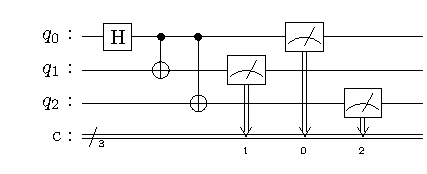
\includegraphics[h]{pdf/example}
        \caption{
            GHZ State
        }
        \label{fig:circuit1}
    \end{figure}


    \section{Efficient Block Encoding of s-Sparse Matrices}



    \bibliographystyle{unsrt}
    \bibliography{references}
\end{document}